\documentclass[11pt,a4paper]{article}
\usepackage[utf8]{inputenc}
\usepackage[T1]{fontenc}
\usepackage[spanish,es-tabla]{babel}
\usepackage[margin=2.2cm]{geometry}
\usepackage{amsmath,amssymb}
\usepackage{booktabs}
\usepackage{graphicx}
\usepackage{float}
\usepackage{subcaption}
\usepackage[hidelinks]{hyperref}

\graphicspath{{./}{results/}{../results/}}

\title{\textbf{Informe Laboratorio 02: Redes Convolucionales 1D para Clasificaci\'on Multiclase (Softmax) y Ordinal (CORAL) en la Escala GDS}}
\author{Laboratorio de Deep Learning (DL-2026-02-L02)}
\date{\today}

\begin{document}

\maketitle
\tableofcontents
\newpage

\section{Resumen Ejecutivo}

En este informe se presenta la implementaci\'on y evaluaci\'on experimental de una arquitectura neuronal \textbf{Conv1D + MLP} (\texttt{Conv1DBackbone}) dise\~nada para predecir el grado de deterioro cognitivo seg\'un la escala \textbf{GDS (\textit{Global Deterioration Scale})} y sus cinco reagrupaciones cl\'inicas (\texttt{GDS\_R1} a \texttt{GDS\_R5}), a partir de una secuencia ordenada de 15 respuestas binarias de orientaci\'on temporal, espacial y top\'onimos locales ($N = 1119$ pacientes).

Sobre el mismo extractor de caracter\'isticas convolucional se comparan tres formulaciones bajo \textbf{validaci\'on cruzada anidada} ($5 \times 3$ folds estratificados en \texttt{GDS\_R1}--\texttt{GDS\_R5}, y $2 \times 2$ folds en \texttt{GDS}) con b\'usqueda interna de hiperpar\'ametros (\texttt{GridSearch} seleccionada por menor MAE ordinal y desempate por mayor QWK):
\begin{enumerate}
    \item \textbf{Conv1D + Softmax} (\texttt{Conv1DSoftmaxNet}): Cabeza lineal de $K$ logits independientes entrenada con entrop\'ia cruzada multiclase (\texttt{CrossEntropyLoss}) y regla de decisi\'on por $\arg\max$.
    \item \textbf{Conv1D + CORAL} (\texttt{Conv1DCoralNet}): Cabeza ordinal (\texttt{CoralLayer}) que proyecta la representaci\'on oculta $h \in \mathbb{R}^H$ a un \'unico puntaje latente escalar $s(x) = w^\top h$ acompa\~nado de $K-1$ umbrales ordenados $b_0 \ge b_1 \ge \dots \ge b_{K-2}$, entrenada mediante entrop\'ia cruzada binaria sobre niveles acumulativos (\texttt{coral\_loss}).
    \item \textbf{Conv1D + CORAL + pesos}: Extensi\'on del modelo CORAL que pondera cada muestra en la funci\'on de p\'erdida seg\'un el \textbf{n\'umero efectivo de muestras} de su clase real ($w_c = \frac{1-\beta}{1-\beta^{n_c}}$, con $\beta = 0.99$) para compensar el desbalance severo entre etapas.
\end{enumerate}

\section{Resultados Experimentales en los 6 Objetivos}

En los Cuadros~\ref{tab:gds} a~\ref{tab:gds_r5} se reporta el desempe\~no externo (media $\pm$ desviaci\'on est\'andar en los folds de prueba) de las tres variantes en los seis objetivos. Se resalta en \textbf{negrita} el mejor valor promedio de cada m\'etrica por objetivo.

\begin{table}[H]
\centering
\caption{Resultados en los folds externos para \textbf{GDS}: Escala original de 7 etapas ($K = 7$: $149 / 500 / 298 / 108 / 42 / 20 / 2$, validaci\'on $2 \times 2$ folds)}
\label{tab:gds}
\resizebox{\textwidth}{!}{%
\begin{tabular}{llccccccc}
\toprule
\textbf{Modelo} & \textbf{HP (Conv, $k$, $h$)} & \textbf{Acc} & \textbf{$\text{F1}_{\text{m}}$} & \textbf{BalAcc} & \textbf{MAE} & \textbf{QWK} & \textbf{Acc$\pm 1$} & \textbf{Err$\ge 2$} \\
\midrule
\textbf{Conv1D + Softmax} & \texttt{16-32, k=3, h=32} & $\mathbf{0.5683 \pm 0.0209}$ & $\mathbf{0.3347 \pm 0.0001}$ & $0.3458 \pm 0.0122$ & $\mathbf{0.4737 \pm 0.0147}$ & $\mathbf{0.7051 \pm 0.0112}$ & $\mathbf{0.9625 \pm 0.0071}$ & $\mathbf{0.0375 \pm 0.0071}$ \\
\textbf{Conv1D + CORAL} & \texttt{16-32, k=3, h=32} & $0.4120 \pm 0.0112$ & $0.2955 \pm 0.0157$ & $0.3684 \pm 0.0599$ & $0.6890 \pm 0.0301$ & $0.6853 \pm 0.0134$ & $0.9088 \pm 0.0144$ & $0.0912 \pm 0.0144$ \\
\textbf{Conv1D + CORAL + pesos} & \texttt{16-32, k=3, h=32} & $0.3369 \pm 0.0095$ & $0.3029 \pm 0.0501$ & $\mathbf{0.4437 \pm 0.0263}$ & $0.7864 \pm 0.0293$ & $0.6783 \pm 0.0066$ & $0.8910 \pm 0.0198$ & $0.1090 \pm 0.0198$ \\
\bottomrule
\end{tabular}%
}
\end{table}

\begin{table}[H]
\centering
\caption{Resultados en los folds externos para \textbf{GDS\_R1}: Reagrupaci\'on 1 ($K = 3$: $\{1,2,3\}\to 1\ [947]$; $\{4,5\}\to 2\ [150]$; $\{6,7\}\to 3\ [22]$)}
\label{tab:gds_r1}
\resizebox{\textwidth}{!}{%
\begin{tabular}{llccccccc}
\toprule
\textbf{Modelo} & \textbf{HP (Conv, $k$, $h$)} & \textbf{Acc} & \textbf{$\text{F1}_{\text{m}}$} & \textbf{BalAcc} & \textbf{MAE} & \textbf{QWK} & \textbf{Acc$\pm 1$} & \textbf{Err$\ge 2$} \\
\midrule
\textbf{Conv1D + Softmax} & \texttt{8-16, k=3, h=32} & $\mathbf{0.8972 \pm 0.0225}$ & $\mathbf{0.7493 \pm 0.0295}$ & $\mathbf{0.7331 \pm 0.0386}$ & $\mathbf{0.1037 \pm 0.0224}$ & $\mathbf{0.6912 \pm 0.0573}$ & $\mathbf{0.9991 \pm 0.0018}$ & $\mathbf{0.0009 \pm 0.0018}$ \\
\textbf{Conv1D + CORAL} & \texttt{8-16, k=3, h=32} & $0.8883 \pm 0.0150$ & $0.6792 \pm 0.0283$ & $0.6810 \pm 0.0477$ & $0.1144 \pm 0.0156$ & $0.6307 \pm 0.0676$ & $0.9973 \pm 0.0022$ & $0.0027 \pm 0.0022$ \\
\textbf{Conv1D + CORAL + pesos} & \texttt{16-32, k=3, h=64} & $0.8767 \pm 0.0151$ & $0.5983 \pm 0.0462$ & $0.6596 \pm 0.0332$ & $0.1269 \pm 0.0168$ & $0.6461 \pm 0.0384$ & $0.9964 \pm 0.0033$ & $0.0036 \pm 0.0033$ \\
\bottomrule
\end{tabular}%
}
\end{table}

\begin{table}[H]
\centering
\caption{Resultados en los folds externos para \textbf{GDS\_R2}: Reagrupaci\'on 2 ($K = 3$: $\{1,2\}\to 1\ [649]$; $\{3\}\to 2\ [298]$; $\{4\text{--}7\}\to 3\ [172]$)}
\label{tab:gds_r2}
\resizebox{\textwidth}{!}{%
\begin{tabular}{llccccccc}
\toprule
\textbf{Modelo} & \textbf{HP (Conv, $k$, $h$)} & \textbf{Acc} & \textbf{$\text{F1}_{\text{m}}$} & \textbf{BalAcc} & \textbf{MAE} & \textbf{QWK} & \textbf{Acc$\pm 1$} & \textbf{Err$\ge 2$} \\
\midrule
\textbf{Conv1D + Softmax} & \texttt{8-16, k=3, h=32} & $0.7247 \pm 0.0354$ & $\mathbf{0.6608 \pm 0.0355}$ & $0.6428 \pm 0.0379$ & $0.2914 \pm 0.0409$ & $0.6915 \pm 0.0572$ & $\mathbf{0.9839 \pm 0.0073}$ & $\mathbf{0.0161 \pm 0.0073}$ \\
\textbf{Conv1D + CORAL} & \texttt{8-16, k=3, h=32} & $\mathbf{0.7319 \pm 0.0232}$ & $0.6494 \pm 0.0280$ & $0.6428 \pm 0.0342$ & $0.2949 \pm 0.0276$ & $0.6831 \pm 0.0440$ & $0.9732 \pm 0.0064$ & $0.0268 \pm 0.0064$ \\
\textbf{Conv1D + CORAL + pesos} & \texttt{8-16, k=3, h=32} & $0.7319 \pm 0.0281$ & $0.6516 \pm 0.0354$ & $\mathbf{0.6497 \pm 0.0428}$ & $\mathbf{0.2905 \pm 0.0284}$ & $\mathbf{0.6987 \pm 0.0394}$ & $0.9777 \pm 0.0028$ & $0.0223 \pm 0.0028$ \\
\bottomrule
\end{tabular}%
}
\end{table}

\begin{table}[H]
\centering
\caption{Resultados en los folds externos para \textbf{GDS\_R3}: Reagrupaci\'on 3 binaria ($K = 2$: $\{1,2,3\}\to 1\ [947]$; $\{4\text{--}7\}\to 3\ [172]$)}
\label{tab:gds_r3}
\resizebox{\textwidth}{!}{%
\begin{tabular}{llccccccc}
\toprule
\textbf{Modelo} & \textbf{HP (Conv, $k$, $h$)} & \textbf{Acc} & \textbf{$\text{F1}_{\text{m}}$} & \textbf{BalAcc} & \textbf{MAE} & \textbf{QWK} & \textbf{Acc$\pm 1$} & \textbf{Err$\ge 2$} \\
\midrule
\textbf{Conv1D + Softmax} & \texttt{8-16, k=3, h=32} & $0.9035 \pm 0.0210$ & $0.7851 \pm 0.0442$ & $0.7479 \pm 0.0380$ & $0.0965 \pm 0.0210$ & $0.5727 \pm 0.0880$ & $\mathbf{1.0000 \pm 0.0000}$ & $\mathbf{0.0000 \pm 0.0000}$ \\
\textbf{Conv1D + CORAL} & \texttt{8-16, k=3, h=32} & $\mathbf{0.9053 \pm 0.0221}$ & $0.7915 \pm 0.0466$ & $0.7562 \pm 0.0408$ & $\mathbf{0.0947 \pm 0.0221}$ & $0.5851 \pm 0.0928$ & $\mathbf{1.0000 \pm 0.0000}$ & $\mathbf{0.0000 \pm 0.0000}$ \\
\textbf{Conv1D + CORAL + pesos} & \texttt{8-16, k=3, h=32} & $0.9044 \pm 0.0161$ & $\mathbf{0.8009 \pm 0.0270}$ & $\mathbf{0.7770 \pm 0.0202}$ & $0.0956 \pm 0.0161$ & $\mathbf{0.6026 \pm 0.0543}$ & $\mathbf{1.0000 \pm 0.0000}$ & $\mathbf{0.0000 \pm 0.0000}$ \\
\bottomrule
\end{tabular}%
}
\end{table}

\begin{table}[H]
\centering
\caption{Resultados en los folds externos para \textbf{GDS\_R4}: Reagrupaci\'on 4 ($K = 3$: $\{1\}\to 1\ [149]$; $\{2,3,4\}\to 2\ [906]$; $\{5,6,7\}\to 3\ [64]$)}
\label{tab:gds_r4}
\resizebox{\textwidth}{!}{%
\begin{tabular}{llccccccc}
\toprule
\textbf{Modelo} & \textbf{HP (Conv, $k$, $h$)} & \textbf{Acc} & \textbf{$\text{F1}_{\text{m}}$} & \textbf{BalAcc} & \textbf{MAE} & \textbf{QWK} & \textbf{Acc$\pm 1$} & \textbf{Err$\ge 2$} \\
\midrule
\textbf{Conv1D + Softmax} & \texttt{8-16, k=3, h=32} & $\mathbf{0.8302 \pm 0.0094}$ & $0.5139 \pm 0.0312$ & $0.5162 \pm 0.0381$ & $\mathbf{0.1698 \pm 0.0094}$ & $0.2930 \pm 0.0508$ & $\mathbf{1.0000 \pm 0.0000}$ & $\mathbf{0.0000 \pm 0.0000}$ \\
\textbf{Conv1D + CORAL} & \texttt{16-32, k=5, h=32} & $0.6971 \pm 0.0267$ & $\mathbf{0.5984 \pm 0.0243}$ & $0.6638 \pm 0.0322$ & $0.3029 \pm 0.0267$ & $\mathbf{0.4001 \pm 0.0291}$ & $\mathbf{1.0000 \pm 0.0000}$ & $\mathbf{0.0000 \pm 0.0000}$ \\
\textbf{Conv1D + CORAL + pesos} & \texttt{16-32, k=5, h=32} & $0.6175 \pm 0.0298$ & $0.5531 \pm 0.0182$ & $\mathbf{0.6827 \pm 0.0135}$ & $0.3825 \pm 0.0298$ & $0.3772 \pm 0.0142$ & $\mathbf{1.0000 \pm 0.0000}$ & $\mathbf{0.0000 \pm 0.0000}$ \\
\bottomrule
\end{tabular}%
}
\end{table}

\begin{table}[H]
\centering
\caption{Resultados en los folds externos para \textbf{GDS\_R5}: Reagrupaci\'on 5 ($K = 3$: $\{1\}\to 1\ [149]$; $\{2,3\}\to 2\ [798]$; $\{4\text{--}7\}\to 3\ [172]$)}
\label{tab:gds_r5}
\resizebox{\textwidth}{!}{%
\begin{tabular}{llccccccc}
\toprule
\textbf{Modelo} & \textbf{HP (Conv, $k$, $h$)} & \textbf{Acc} & \textbf{$\text{F1}_{\text{m}}$} & \textbf{BalAcc} & \textbf{MAE} & \textbf{QWK} & \textbf{Acc$\pm 1$} & \textbf{Err$\ge 2$} \\
\midrule
\textbf{Conv1D + Softmax} & \texttt{8-16, k=3, h=32} & $\mathbf{0.7748 \pm 0.0066}$ & $0.5037 \pm 0.0143$ & $0.5095 \pm 0.0178$ & $\mathbf{0.2252 \pm 0.0066}$ & $0.4274 \pm 0.0320$ & $\mathbf{1.0000 \pm 0.0000}$ & $\mathbf{0.0000 \pm 0.0000}$ \\
\textbf{Conv1D + CORAL} & \texttt{8-16, k=3, h=32} & $0.6381 \pm 0.0430$ & $\mathbf{0.5783 \pm 0.0320}$ & $0.6330 \pm 0.0371$ & $0.3664 \pm 0.0460$ & $\mathbf{0.4893 \pm 0.0409}$ & $0.9955 \pm 0.0057$ & $0.0045 \pm 0.0057$ \\
\textbf{Conv1D + CORAL + pesos} & \texttt{16-32, k=3, h=64} & $0.5630 \pm 0.0338$ & $0.5439 \pm 0.0354$ & $\mathbf{0.6371 \pm 0.0335}$ & $0.4424 \pm 0.0373$ & $0.4694 \pm 0.0424$ & $0.9946 \pm 0.0052$ & $0.0054 \pm 0.0052$ \\
\bottomrule
\end{tabular}%
}
\end{table}

\newpage
\section{Gr\'aficos Comparativos y Matrices de Confusi\'on}

\subsection{Comparaci\'on Global por M\'etrica en los 6 Objetivos}

La Figura~\ref{fig:comp_6_obj} resume visualmente las m\'etricas ordinales (\texttt{MAE}, \texttt{Errores Graves}, \texttt{QWK}) y multiclase (\texttt{F1 Macro}, \texttt{Balanced Accuracy}, \texttt{Accuracy}) para los tres modelos evaluados.

\begin{figure}[H]
    \centering
    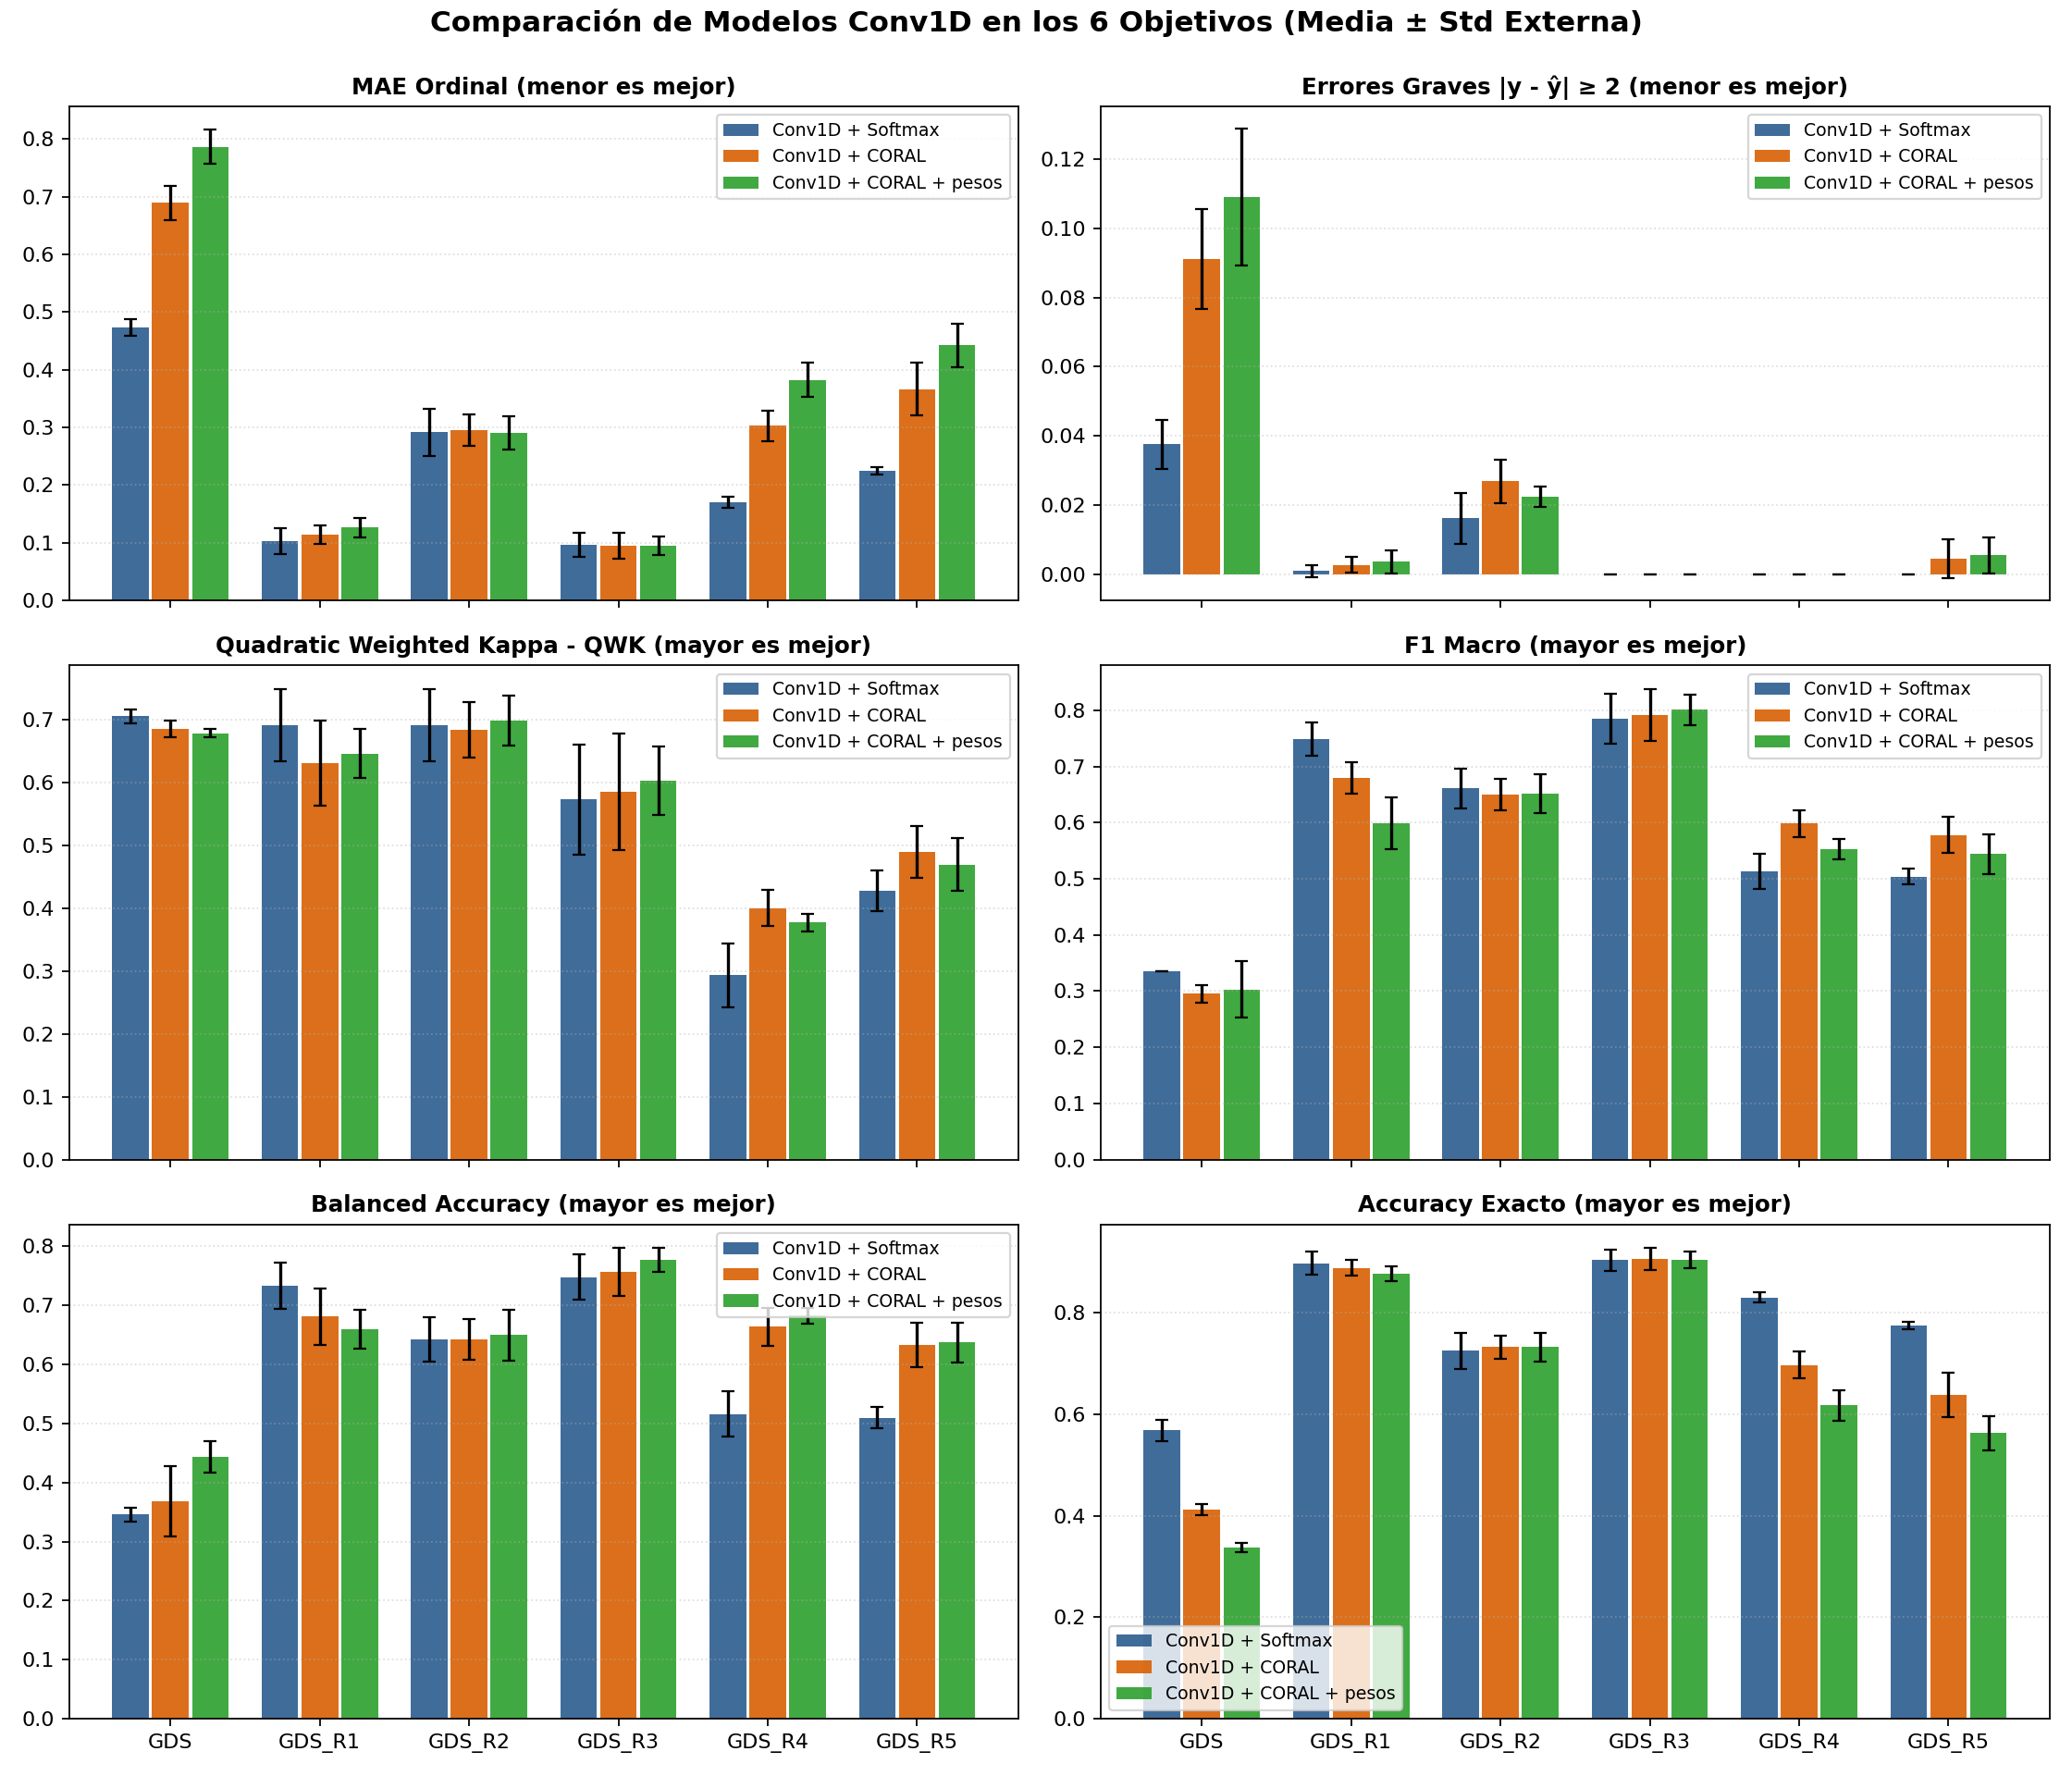
\includegraphics[width=0.98\textwidth]{comparacion_metricas_6_objetivos.png}
    \caption{Comparaci\'on de \texttt{Conv1D + Softmax}, \texttt{Conv1D + CORAL} y \texttt{Conv1D + CORAL + pesos} a lo largo de los 6 objetivos (media $\pm 1$ desviaci\'on est\'andar en los folds externos).}
    \label{fig:comp_6_obj}
\end{figure}

\begin{figure}[H]
    \centering
    \begin{subfigure}[b]{0.48\textwidth}
        \centering
        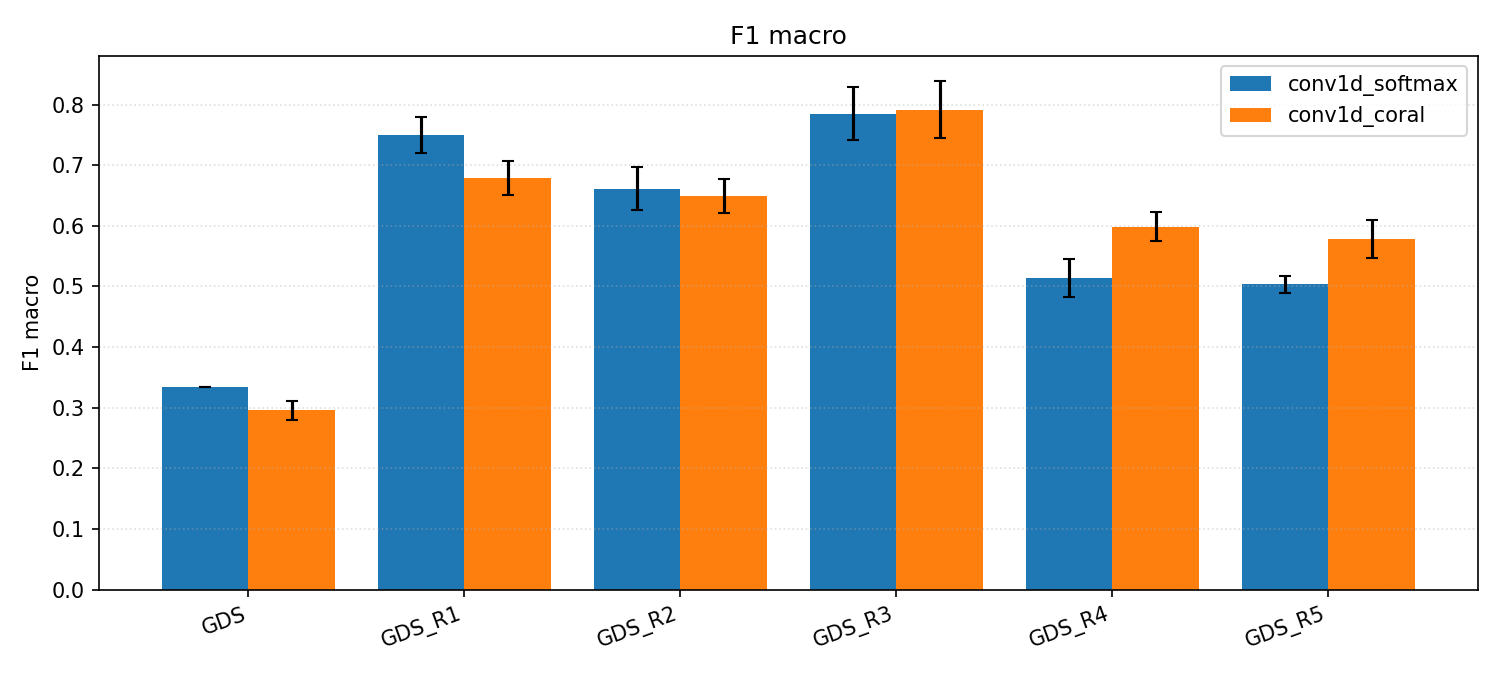
\includegraphics[width=\textwidth]{barras_f1.png}
        \caption{F1 Macro (Softmax vs.\ CORAL sin pesos).}
    \end{subfigure}
    \hfill
    \begin{subfigure}[b]{0.48\textwidth}
        \centering
        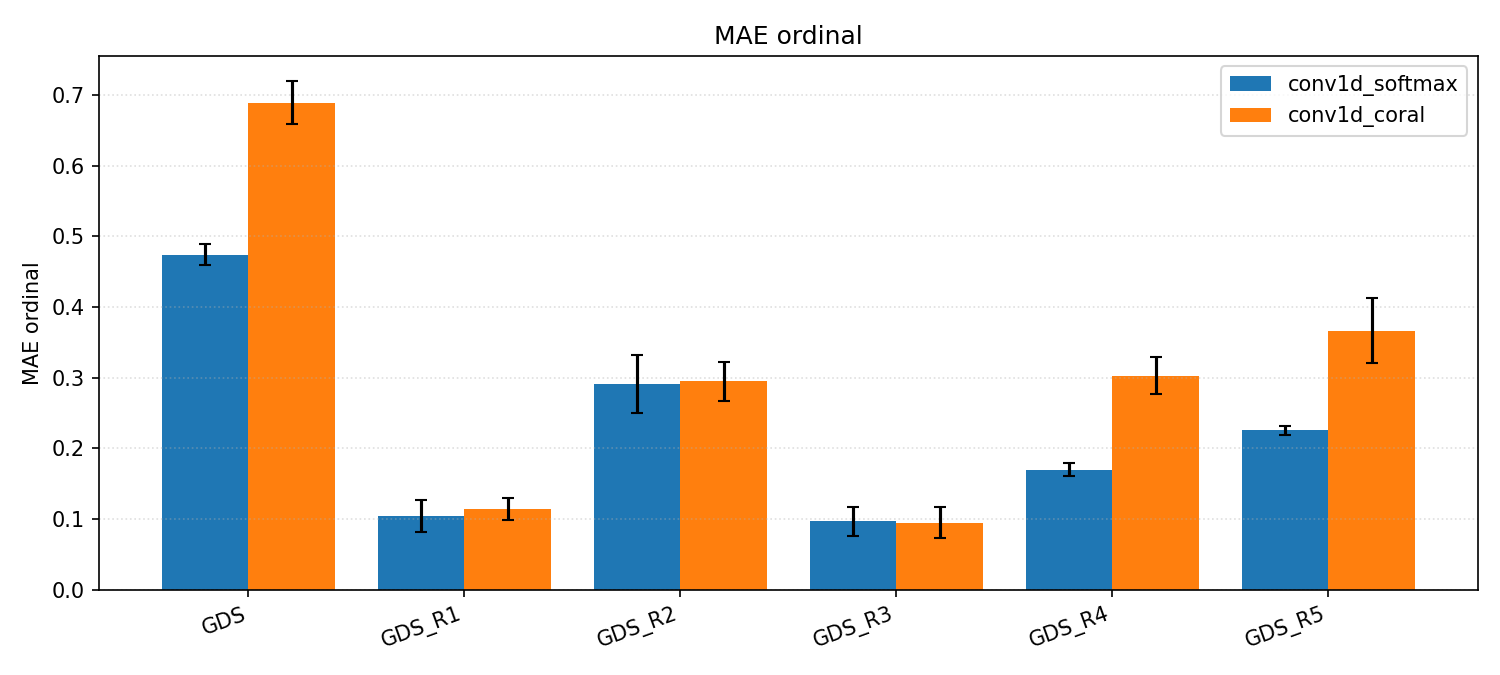
\includegraphics[width=\textwidth]{barras_mae.png}
        \caption{MAE Ordinal (Softmax vs.\ CORAL sin pesos).}
    \end{subfigure}
    \caption{Gr\'aficos de barras directos generados por \texttt{ReportWriter} en \texttt{results/}.}
    \label{fig:barras_directas}
\end{figure}

\subsection{Matrices de Confusi\'on del \'Ultimo Fold Externo}

Las Figuras~\ref{fig:cm_part1} y~\ref{fig:cm_part2} contrastan lado a lado las matrices de confusi\'on del \'ultimo fold externo de prueba para las tres variantes en cada uno de los seis objetivos.

\begin{figure}[H]
    \centering
    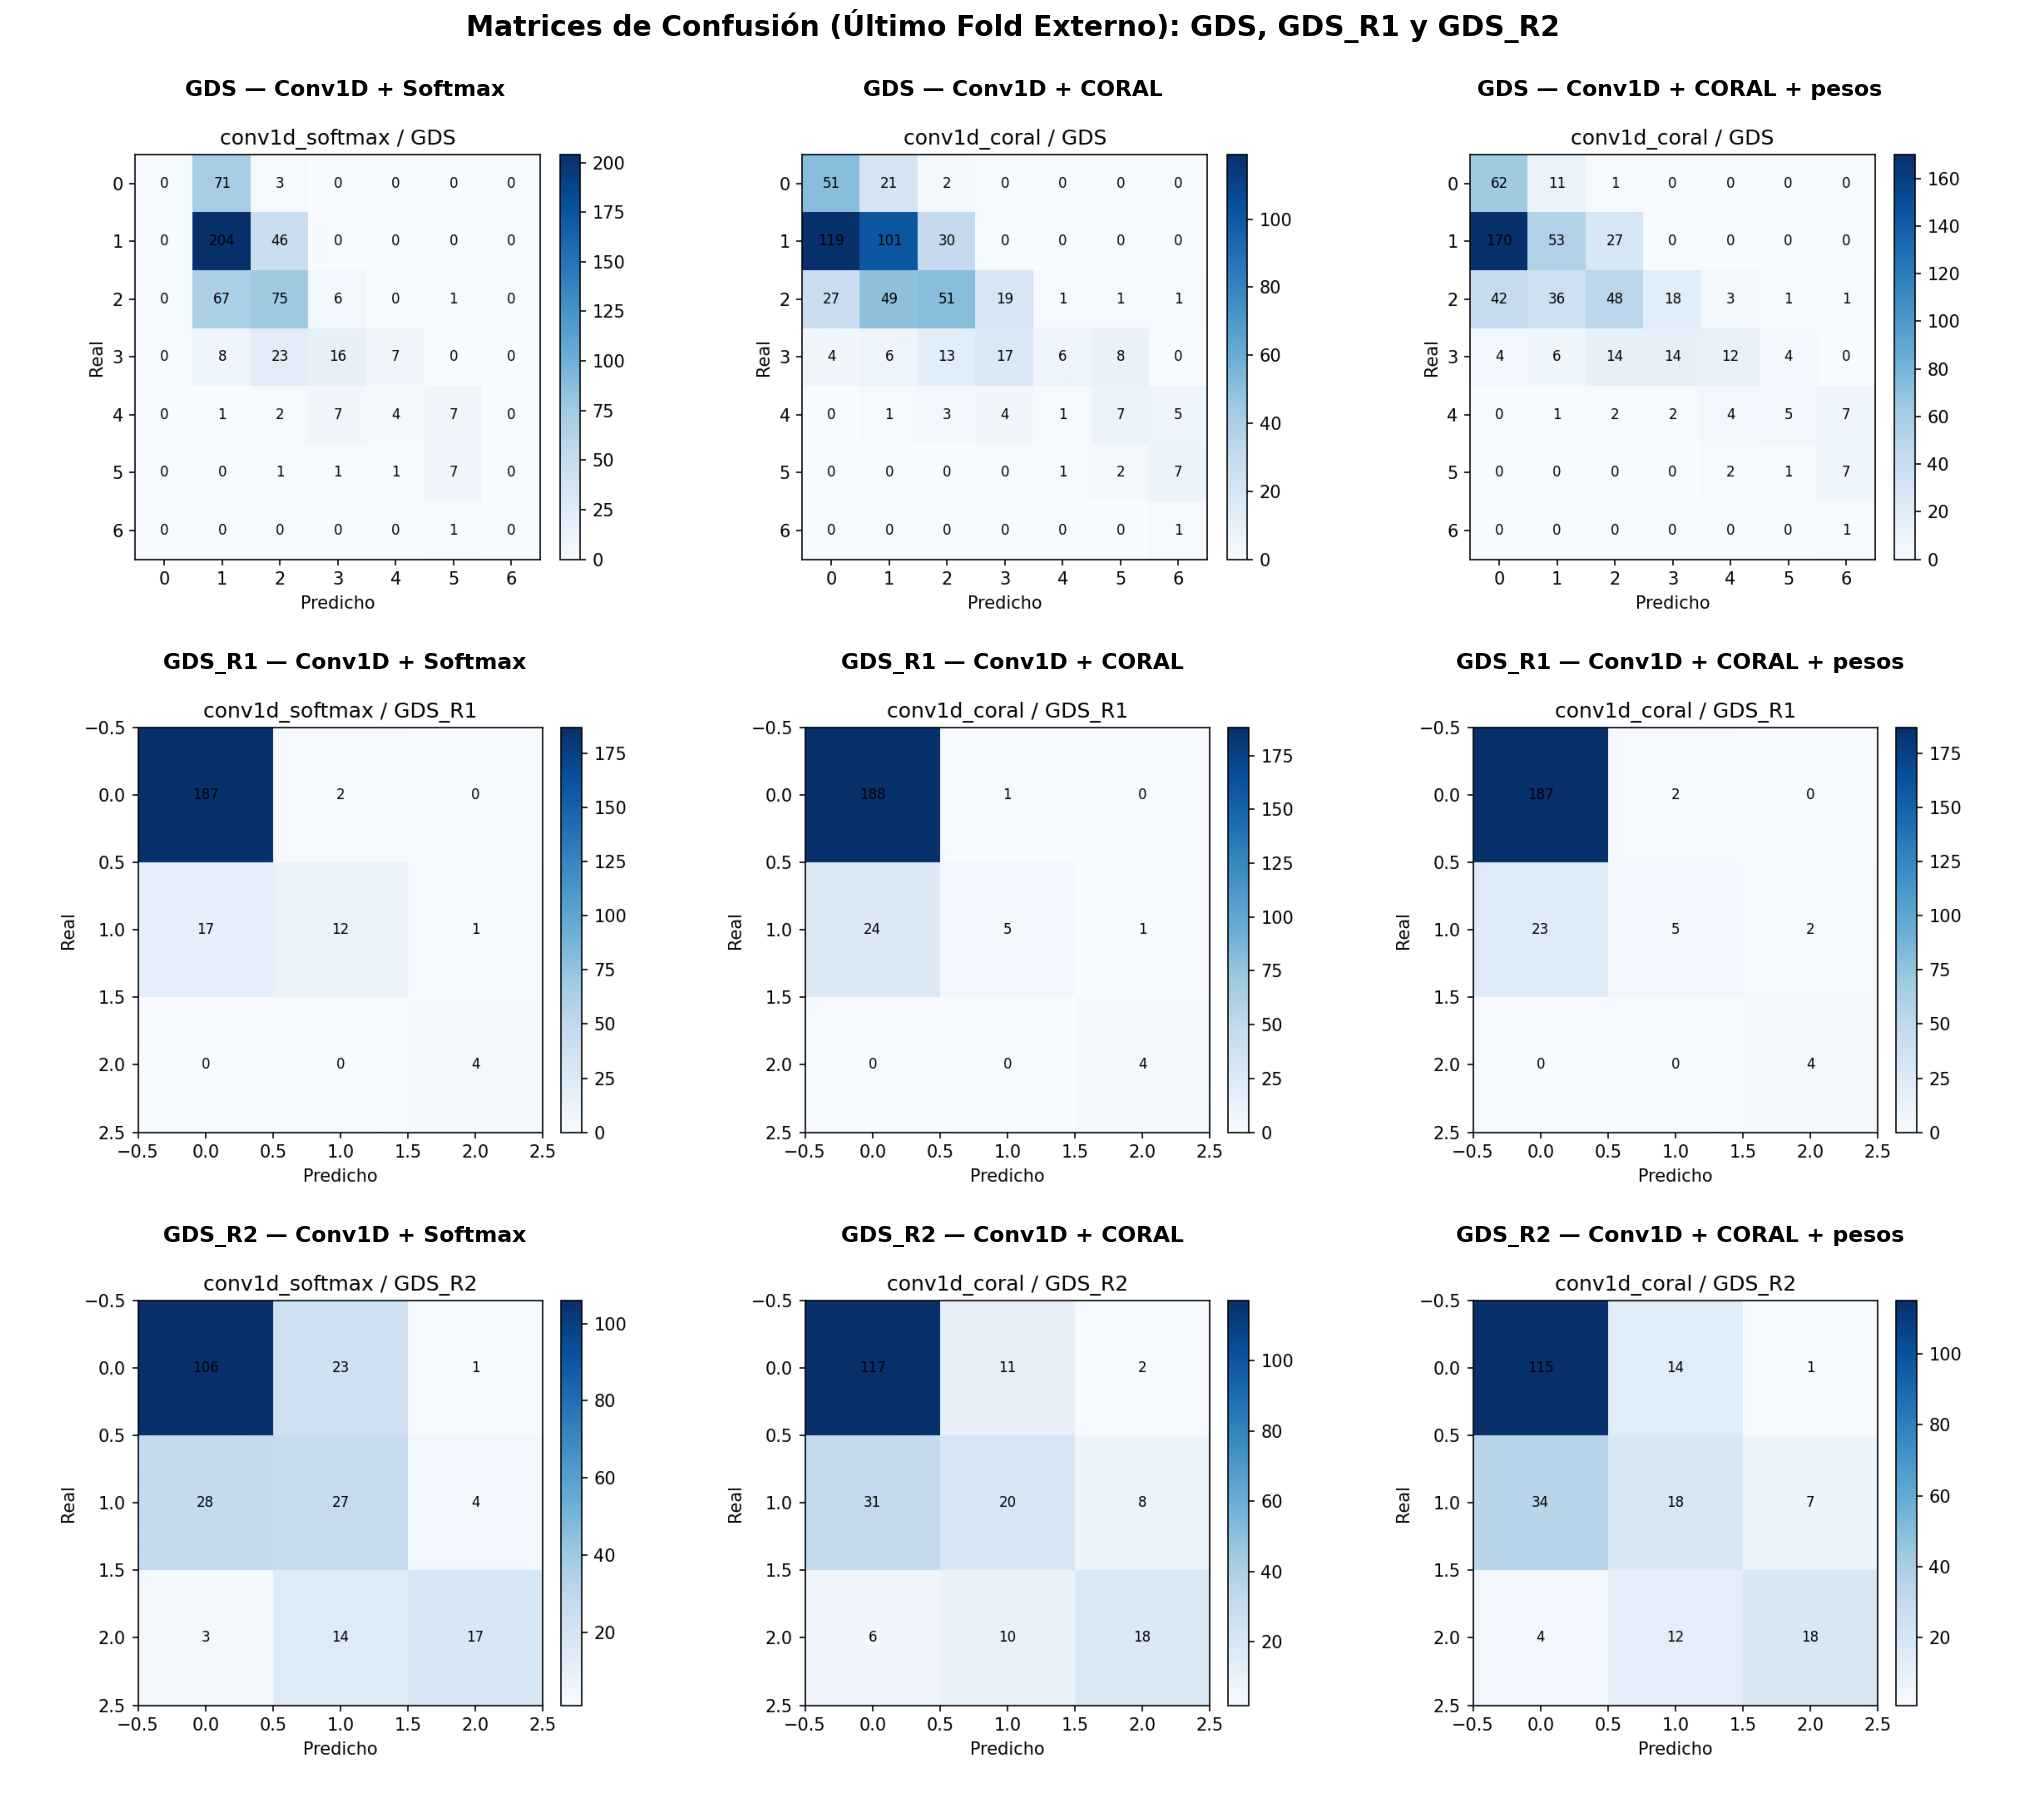
\includegraphics[width=0.96\textwidth]{comparacion_confusion_GDS_a_R2.png}
    \caption{Matrices de confusi\'on del \'ultimo fold externo para \texttt{GDS}, \texttt{GDS\_R1} y \texttt{GDS\_R2}.}
    \label{fig:cm_part1}
\end{figure}

\begin{figure}[H]
    \centering
    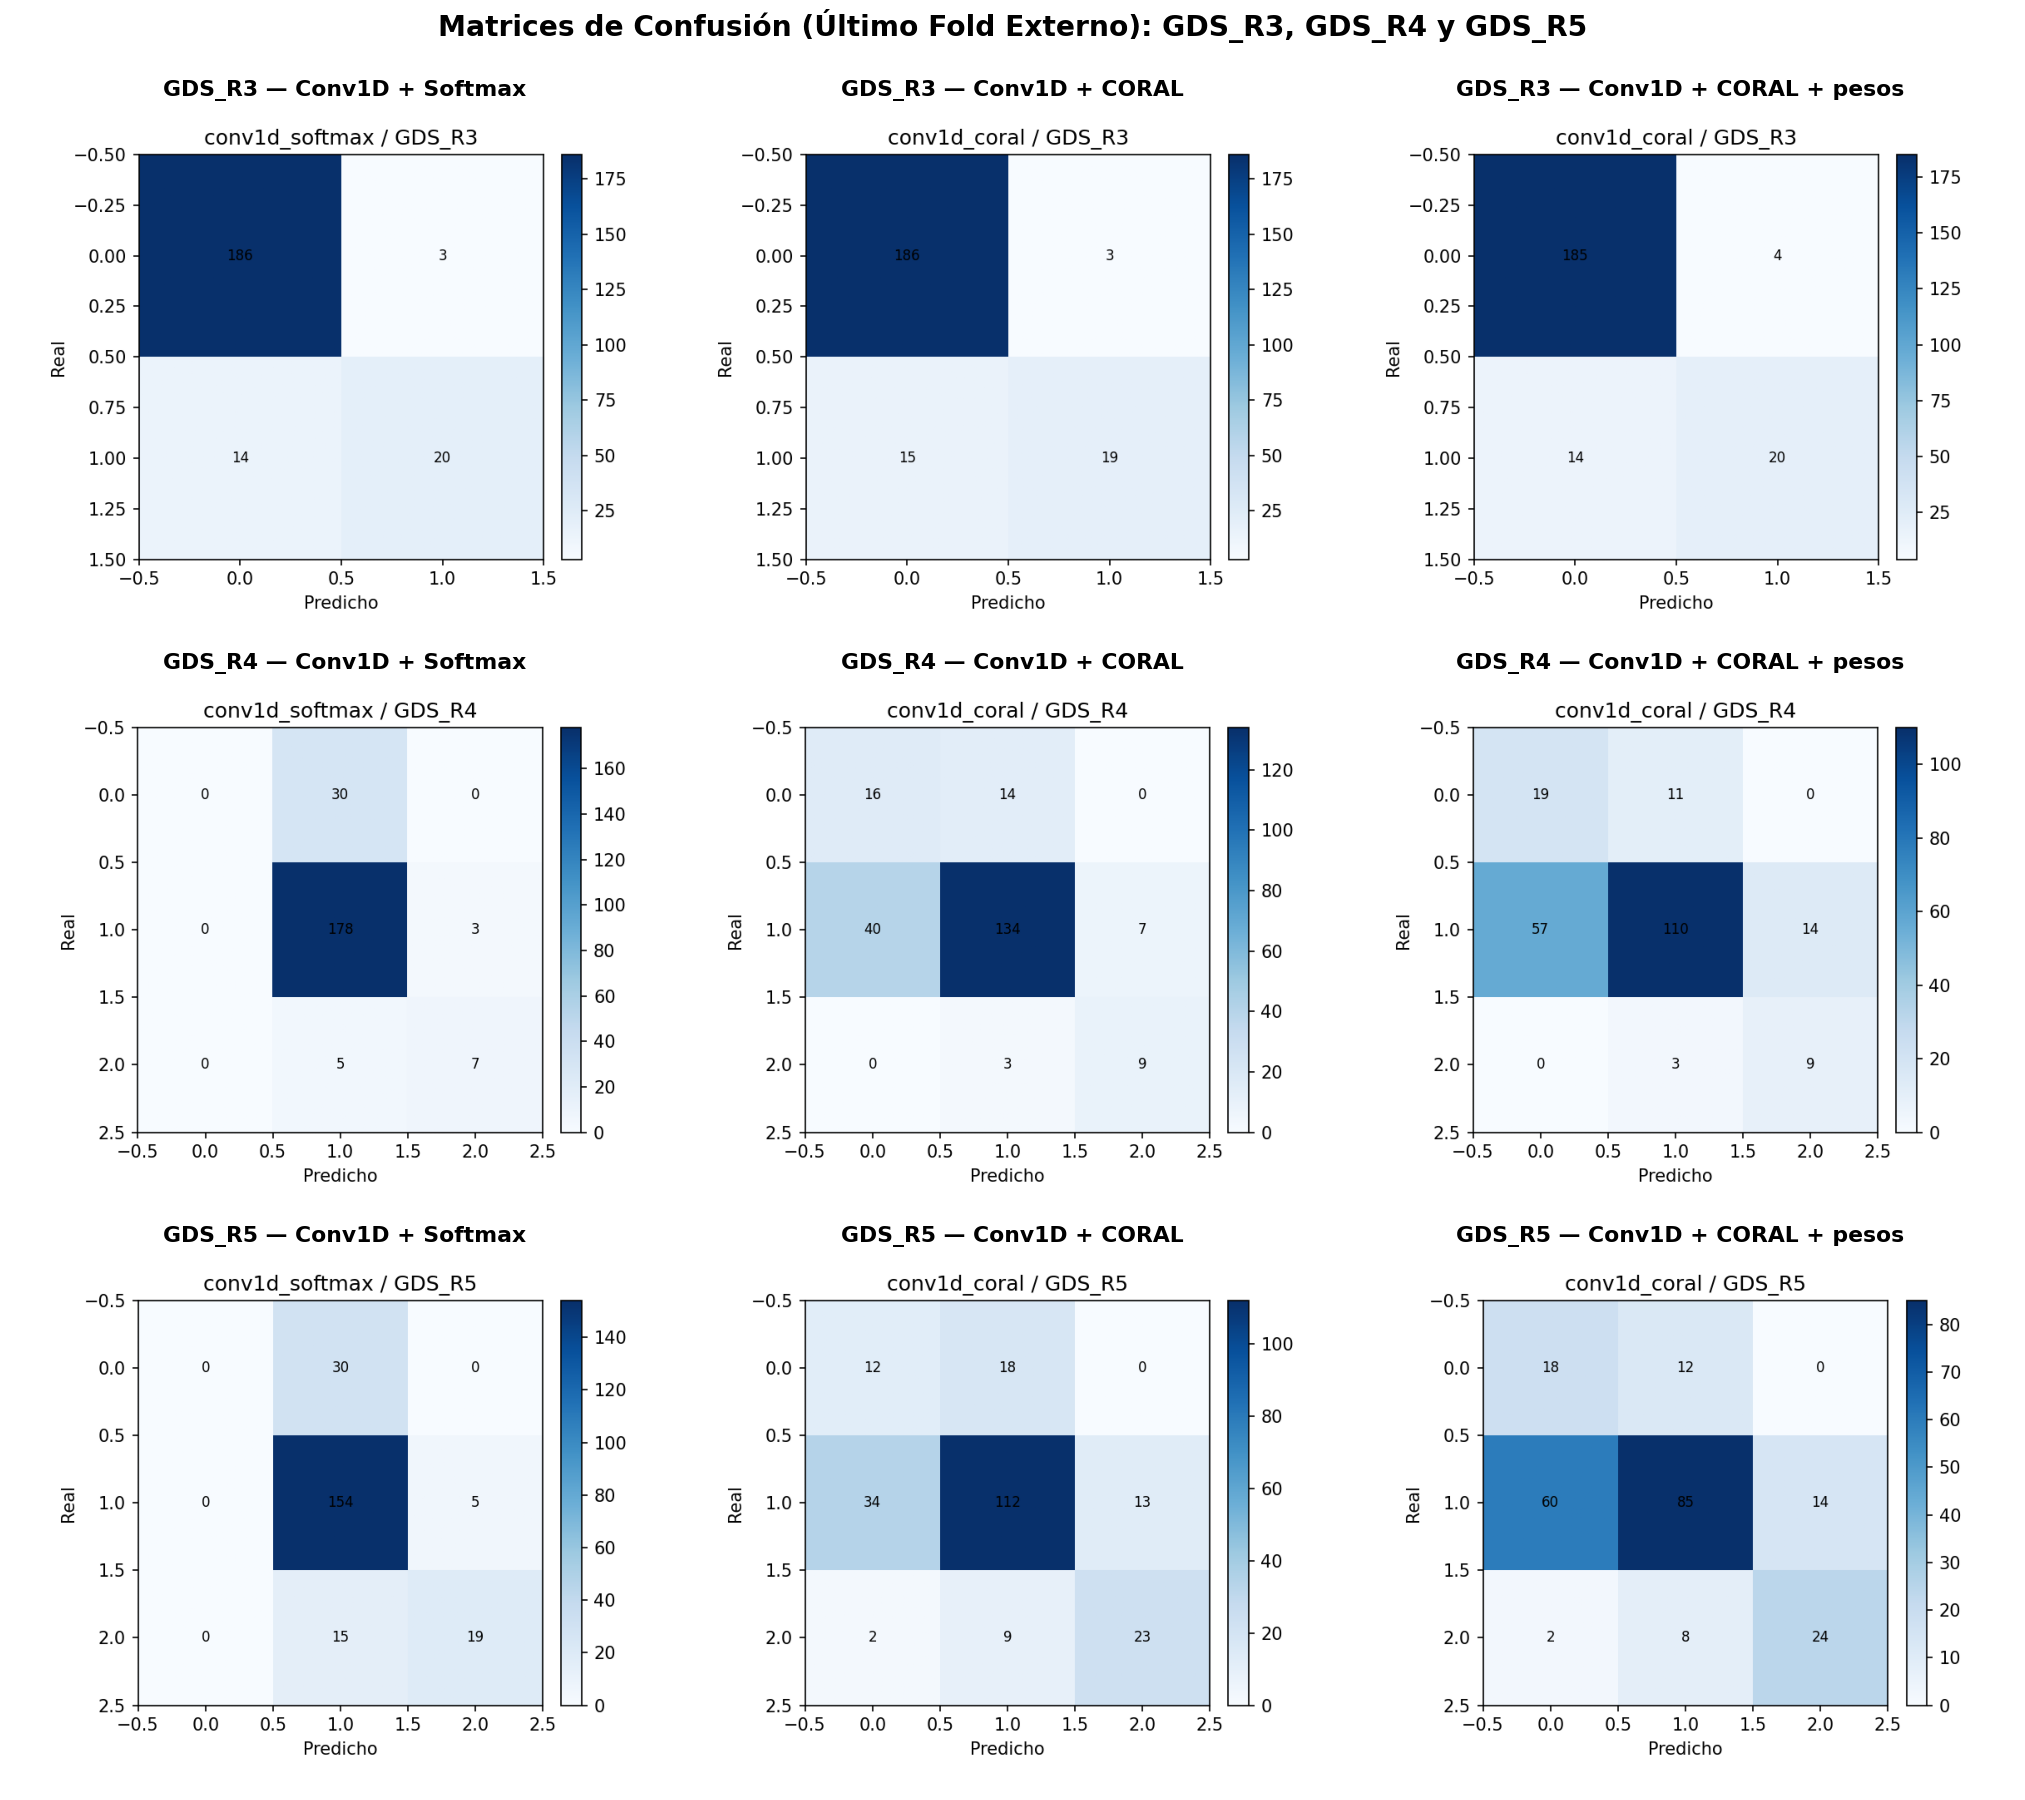
\includegraphics[width=0.96\textwidth]{comparacion_confusion_R3_a_R5.png}
    \caption{Matrices de confusi\'on del \'ultimo fold externo para \texttt{GDS\_R3}, \texttt{GDS\_R4} y \texttt{GDS\_R5}.}
    \label{fig:cm_part2}
\end{figure}

\newpage
\section{Respuestas a las Preguntas del Informe}

\subsection{1. ?`Qu\'e patrones locales puede aprender un kernel de tama\~no 3 sobre los 15 \'items?}

En \texttt{src/config.py}, los 15 atributos binarios (\texttt{FEATURE\_COLUMNS}) est\'an ordenados siguiendo una estructura cl\'inica dividida en tres subgrupos contiguos:
\begin{itemize}
    \item \textbf{Orientaci\'on temporal (posiciones 0--3)}: \texttt{D\'ia}, \texttt{Mes}, \texttt{A\~no}, \texttt{Estaci\'on}.
    \item \textbf{Orientaci\'on espacial (posiciones 4--7)}: \texttt{Pa\'is}, \texttt{Ciudad}, \texttt{CalleLugar}, \texttt{NumeroPiso}.
    \item \textbf{Top\'onimos locales (posiciones 8--14)}: \texttt{Miguel2}, \texttt{Gonz\'alez2}, \texttt{Avenida2}, \texttt{Imperial2}, \texttt{A682}, \texttt{Caldera2}, \texttt{Copiapo2}.
\end{itemize}

Un filtro convolucional 1D de tama\~no $k = 3$ con $\text{padding} = 1$ y $\text{stride} = 1$ (\texttt{Conv1DBlock}) recorre cada terna de respuestas vecinas $(x_{i-1}, x_i, x_{i+1})$:
\begin{enumerate}
    \item \textbf{En la primera capa convolucional}: cada canal detecta \textbf{co-ocurrencias locales de aciertos o fallos} dentro de un mismo bloque cognitivo, tales como fallar simult\'aneamente \texttt{D\'ia--Mes--A\~no} (desorientaci\'on temporal completa), fallar el par o triplete espacial \texttt{Ciudad--CalleLugar--NumeroPiso}, detectar transiciones en los bordes entre orientaci\'on temporal y espacial (\texttt{Estaci\'on--Pa\'is--Ciudad}), o identificar r\'afagas de errores consecutivos en los top\'onimos locales.
    \item \textbf{En la segunda capa convolucional}: al aplicar un segundo kernel de ancho $k = 3$ sobre las caracter\'isticas de la primera capa, el \textbf{campo receptivo efectivo se expande a $3 + (3 - 1) = 5$ \'items consecutivos}, lo que permite resumir el estado completo del bloque temporal (4 \'items) o espacial (4 \'items) antes del clasificador MLP.
\end{enumerate}

\subsection{2. ?`Qu\'e pasa con la Conv1D si se permutan las columnas de entrada? ?`Y con una MLP?}

\begin{itemize}
    \item \textbf{En una MLP (\texttt{nn.Linear})}: Una capa densa calcula $h = \phi(Wx + b)$ conectando cada neurona oculta con las 15 entradas de manera global. Si se aplica una permutaci\'on $\Pi$ a las columnas de entrada ($x' = \Pi x$), ello equivale a permutar las columnas de la matriz de pesos inicial ($W' = W\Pi^\top$). Dado que la inicializaci\'on de los pesos es independiente e id\'enticamente distribuida para cada entrada, el espacio de hip\'otesis y la trayectoria de optimizaci\'on son \textbf{invariantes al orden de las columnas}.
    \item \textbf{En una red \texttt{Conv1D}}: La convoluci\'on 1D impone un sesgo inductivo de \textbf{localidad secuencial} (ventana restringida de tama\~no $k=3$) y \textbf{compartici\'on de pesos} (\textit{weight sharing}). Si se permutan arbitrariamente las columnas (por ejemplo, mezclando \texttt{D\'ia}, \texttt{Copiapo2} y \texttt{Pa\'is}), se rompe la contig\"uidad sem\'antica de los tres subgrupos cognitivos y las ventanas de tama\~no 3 pasan a combinar atributos no relacionados. Por lo tanto, \textbf{la \texttt{Conv1D} no es invariante a permutaciones} y su rendimiento depende directamente del orden de \texttt{FEATURE\_COLUMNS}.
\end{itemize}

\subsection{3. ?`Por qu\'e se usa \texttt{Flatten} en lugar de un pooling global?}

La salida de los bloques convolucionales sobre la secuencia de largo $L = 15$ tiene dimensi\'on $(B, C_{\text{out}}, 15)$.
\begin{itemize}
    \item Si se aplicara un \textbf{pooling global} (\texttt{AdaptiveAvgPool1d(1)} o \texttt{AdaptiveMaxPool1d(1)}), se colapsar\'ia la dimensi\'on posicional a $(B, C_{\text{out}})$, generando \textbf{invarianza a la posici\'on}: la capa densa posterior sabr\'ia que se activ\'o un patr\'on de error, pero perder\'ia por completo la informaci\'on de \textbf{en qu\'e \'item del test ocurri\'o} (no tiene el mismo peso cl\'inico fallar en \texttt{A\~no} o \texttt{Pa\'is} que fallar en un top\'onimo local).
    \item Al emplear \textbf{\texttt{nn.Flatten()}}, se preserva el mapa posicional completo en un vector de tama\~no $C_{\text{out}} \times 15$ ($480$ o $240$ caracter\'isticas), permitiendo que el \texttt{MLPBlock} pondere espec\'ificamente qu\'e filtro se activ\'o y en qu\'e posici\'on exacta de la secuencia.
\end{itemize}

\subsection{4. ?`C\'omo garantiza CORAL la consistencia ordinal?}

Si los $K-1$ umbrales acumulativos $P(Y > k \mid x)$ se modelaran con vectores de pesos independientes $z_k(x) = w_k^\top h + b_k$, los hiperplanos podr\'ian intersectarse y producir contradicciones de rango ($\hat{P}(Y > k \mid x) > \hat{P}(Y > k-1 \mid x)$).

\texttt{CoralLayer} (\texttt{src/models/coral.py}) garantiza la \textbf{consistencia de rango} mediante dos restricciones estructurales:
\begin{enumerate}
    \item \textbf{Direcci\'on de proyecci\'on compartida ($w$)}: Una \'unica proyecci\'on lineal sin sesgo (\texttt{nn.Linear(input\_size, 1, bias=False)}) calcula el puntaje escalar latente $s(x) = w^\top h$, forzando que las $K-1$ fronteras de decisi\'on sean hiperplanos paralelos.
    \item \textbf{Sesgos ordenados decrecientes ($b_0 \ge b_1 \ge \dots \ge b_{K-2}$)}: A partir de un sesgo inicial $b_0$ y $K-2$ par\'ametros $\delta_1, \dots, \delta_{K-2}$, las diferencias entre umbrales consecutivos se restringen a ser positivas mediante la funci\'on $\text{softplus}(\delta_j) = \ln(1 + e^{\delta_j}) > 0$ y se acumulan con \texttt{cumsum}:
    \begin{equation}
        b_k = b_0 - \sum_{j=1}^{k} \text{softplus}(\delta_j) \implies z_0(x) \ge z_1(x) \ge \dots \ge z_{K-2}(x) \quad \forall x.
    \end{equation}
    Dado que la funci\'on sigmoide $\sigma(z)$ es estrictamente creciente, las probabilidades acumulativas satisfacen siempre:
    \begin{equation}
        \hat{P}(Y > 0 \mid x) \ge \hat{P}(Y > 1 \mid x) \ge \dots \ge \hat{P}(Y > K-2 \mid x).
    \end{equation}
\end{enumerate}

\subsection{5. ?`En qu\'e objetivos CORAL mejora MAE / errores graves frente a Softmax?}

A partir de los Cuadros~\ref{tab:gds}--\ref{tab:gds_r5} y las matrices de confusi\'on (Figuras~\ref{fig:cm_part1} y~\ref{fig:cm_part2}), se identifican tres reg\'imenes:
\begin{enumerate}
    \item \textbf{Mejora directa en \texttt{MAE}, \texttt{QWK}, \texttt{Accuracy} y \texttt{Balanced Accuracy} (\texttt{GDS\_R2} y \texttt{GDS\_R3})}:
    \begin{itemize}
        \item En \textbf{\texttt{GDS\_R3}}, \texttt{Conv1D + CORAL} supera a \texttt{Softmax} en todas las m\'etricas: reduce el \texttt{MAE} de $0.0965$ a $\mathbf{0.0947}$, mantiene $\mathbf{0.0000}$ de errores graves, y mejora \texttt{Acc} ($0.9053$ vs.\ $0.9035$), \texttt{F1} ($0.7915$ sin pesos y $\mathbf{0.8009}$ con pesos vs.\ $0.7851$), \texttt{BalAcc} ($\mathbf{0.7770}$ vs.\ $0.7479$) y \texttt{QWK} ($\mathbf{0.6026}$ vs.\ $0.5727$).
        \item En \textbf{\texttt{GDS\_R2}} (objetivo principal por defecto), \texttt{Conv1D + CORAL + pesos} alcanza el \textbf{menor \texttt{MAE} global ($\mathbf{0.2905}$ vs.\ $0.2914$ de Softmax)}, el \textbf{mayor \texttt{QWK} ($\mathbf{0.6987}$ vs.\ $0.6915$)}, el \textbf{mayor \texttt{Accuracy} ($\mathbf{0.7319}$ vs.\ $0.7247$)} y el \textbf{mayor \texttt{Balanced Accuracy} ($\mathbf{0.6497}$ vs.\ $0.6428$)}.
    \end{itemize}
    \item \textbf{Prevenci\'on del colapso a la clase central y mejora de \texttt{QWK}, \texttt{F1 Macro} y \texttt{Balanced Accuracy} (\texttt{GDS\_R4} y \texttt{GDS\_R5})}:
    \begin{itemize}
        \item En \textbf{\texttt{GDS\_R4}} ($81\%$ en la clase central 2) y \textbf{\texttt{GDS\_R5}} ($71.3\%$ en la clase central 2), \texttt{Softmax} colapsa hacia la clase mayoritaria central, obteniendo un \texttt{Balanced Accuracy} cercano al azar ($0.5162$ y $0.5095$) y bajo \texttt{QWK} ($0.2930$ en \texttt{GDS\_R4}).
        \item \texttt{Conv1D + CORAL} mantiene $\mathbf{0.0000}$ errores graves en \texttt{GDS\_R4} y eleva sustancialmente el \textbf{\texttt{QWK}} ($0.4001$ vs.\ $0.2930$ en \texttt{GDS\_R4}; $0.4893$ vs.\ $0.4274$ en \texttt{GDS\_R5}), el \textbf{\texttt{F1 Macro}} ($0.5984$ vs.\ $0.5139$ en \texttt{GDS\_R4}; $0.5783$ vs.\ $0.5037$ en \texttt{GDS\_R5}) y el \textbf{\texttt{Balanced Accuracy}} ($0.6638$ vs.\ $0.5162$ en \texttt{GDS\_R4}; $0.6330$ vs.\ $0.5095$ en \texttt{GDS\_R5}).
    \end{itemize}
    \item \textbf{Comportamiento en \texttt{GDS} de 7 clases ($2 \times 2$ folds)}:
    Al entrenarse con solo 2 folds externos en 20 \'epocas, los 6 umbrales acoplados sobre un \'unico escalar $s(x)=w^\top h$ tienen menor flexibilidad que los 7 vectores independientes de \texttt{Softmax}, por lo que \texttt{Softmax} logra menor \texttt{MAE} ($0.4737$ vs.\ $0.6890$), aunque ignora por completo las etapas extremas 1 y 7, mientras que \texttt{CORAL + pesos} s\'i las recupera y alcanza el mayor \texttt{Balanced Accuracy} ($\mathbf{0.4437}$ vs.\ $0.3458$).
\end{enumerate}

\subsection{6. ?`Qu\'e efecto tienen los pesos por n\'umero efectivo en las clases raras?}

Los pesos por n\'umero efectivo de muestras de Cui et al.\ (\texttt{effective\_number\_weights}):
\begin{equation}
    w_c = \frac{1 - \beta}{1 - \beta^{n_c}}, \qquad \beta = 0.99,
\end{equation}
normalizados a media unitaria, incrementan la contribuci\'on al gradiente de las clases minoritarias. Sus efectos principales son:
\begin{enumerate}
    \item \textbf{Incremento consistente del recall promedio por clase (\texttt{Balanced Accuracy}) en 5 de los 6 objetivos}:
    \texttt{GDS} sube de $0.3684$ a $\mathbf{0.4437}$ ($+9.8$ puntos sobre Softmax); \texttt{GDS\_R2} sube a $\mathbf{0.6497}$ (mejorando tambi\'en \texttt{MAE} a $\mathbf{0.2905}$ y \texttt{QWK} a $\mathbf{0.6987}$); \texttt{GDS\_R3} sube a $\mathbf{0.7770}$ (y \texttt{F1 Macro} a $\mathbf{0.8009}$); \texttt{GDS\_R4} sube a $\mathbf{0.6827}$ ($+16.7$ puntos sobre Softmax); y \texttt{GDS\_R5} sube a $\mathbf{0.6371}$.
    \item \textbf{Compromiso (\textit{trade-off}) entre sensibilidad en extremos y error absoluto global}:
    En objetivos con desbalance moderado (\texttt{GDS\_R2} y \texttt{GDS\_R3}), la ponderaci\'on mejora simult\'aneamente las m\'etricas macro y ordinales. En objetivos con desbalance extremo en los bordes (\texttt{GDS}, \texttt{GDS\_R4} y \texttt{GDS\_R5}), forzar al modelo a detectar las clases raras reduce el colapso hacia la clase mayoritaria pero introduce m\'as falsos positivos hacia las clases extremas, reduciendo el \texttt{Accuracy} exacto y aumentando el \texttt{MAE} promedio.
\end{enumerate}

\end{document}
